\documentclass{article}\usepackage[]{graphicx}\usepackage[]{color}
%% maxwidth is the original width if it is less than linewidth
%% otherwise use linewidth (to make sure the graphics do not exceed the margin)
\makeatletter
\def\maxwidth{ %
  \ifdim\Gin@nat@width>\linewidth
    \linewidth
  \else
    \Gin@nat@width
  \fi
}
\makeatother

\definecolor{fgcolor}{rgb}{0.345, 0.345, 0.345}
\newcommand{\hlnum}[1]{\textcolor[rgb]{0.686,0.059,0.569}{#1}}%
\newcommand{\hlstr}[1]{\textcolor[rgb]{0.192,0.494,0.8}{#1}}%
\newcommand{\hlcom}[1]{\textcolor[rgb]{0.678,0.584,0.686}{\textit{#1}}}%
\newcommand{\hlopt}[1]{\textcolor[rgb]{0,0,0}{#1}}%
\newcommand{\hlstd}[1]{\textcolor[rgb]{0.345,0.345,0.345}{#1}}%
\newcommand{\hlkwa}[1]{\textcolor[rgb]{0.161,0.373,0.58}{\textbf{#1}}}%
\newcommand{\hlkwb}[1]{\textcolor[rgb]{0.69,0.353,0.396}{#1}}%
\newcommand{\hlkwc}[1]{\textcolor[rgb]{0.333,0.667,0.333}{#1}}%
\newcommand{\hlkwd}[1]{\textcolor[rgb]{0.737,0.353,0.396}{\textbf{#1}}}%

\usepackage{framed}
\makeatletter
\newenvironment{kframe}{%
 \def\at@end@of@kframe{}%
 \ifinner\ifhmode%
  \def\at@end@of@kframe{\end{minipage}}%
  \begin{minipage}{\columnwidth}%
 \fi\fi%
 \def\FrameCommand##1{\hskip\@totalleftmargin \hskip-\fboxsep
 \colorbox{shadecolor}{##1}\hskip-\fboxsep
     % There is no \\@totalrightmargin, so:
     \hskip-\linewidth \hskip-\@totalleftmargin \hskip\columnwidth}%
 \MakeFramed {\advance\hsize-\width
   \@totalleftmargin\z@ \linewidth\hsize
   \@setminipage}}%
 {\par\unskip\endMakeFramed%
 \at@end@of@kframe}
\makeatother

\definecolor{shadecolor}{rgb}{.97, .97, .97}
\definecolor{messagecolor}{rgb}{0, 0, 0}
\definecolor{warningcolor}{rgb}{1, 0, 1}
\definecolor{errorcolor}{rgb}{1, 0, 0}
\newenvironment{knitrout}{}{} % an empty environment to be redefined in TeX

\usepackage{alltt}
\usepackage[utf8]{inputenc}
\usepackage[american]{babel}
\usepackage{graphicx}
\usepackage{amsmath}
\usepackage{amsthm}
\usepackage{amssymb}
\usepackage{natbib}
\usepackage{hyperref}
\usepackage[nogin]{Sweave}

\setlength{\textwidth}{6.25in}
\setlength{\textheight}{8.75in}
\setlength{\evensidemargin}{0in}
\setlength{\oddsidemargin}{0in}
\setlength{\topmargin}{-.35in}
\setlength{\parskip}{.1in}  
\setlength{\parindent}{0.0in}  

\setcounter{tocdepth}{1}
\setcounter{secnumdepth}{1}

\newcommand{\R}{\textsf{R}}
\newcommand{\code}[1]{\texttt{#1}}

\SweaveOpts{eps=FALSE,keep.source=TRUE}

\newtheoremstyle{exercise}%
		{\topsep}	%      Space above
		{\topsep}	%      Space below    
		{}		%      Body font
		{} % Indent amount (empty = no indent, \parindent = para indent)
		{\bfseries}	% Thm head font
		{.}		% Punctuation after thm head
		{.5em}	 % Space after thm head (\newline = linebreak)
		{\thmname{#1}\thmnumber{ #2}\thmnote{ #3}} % Thm head spec
\theoremstyle{exercise}
\newtheorem{exercise}{Exercise}
\newtheorem{challenge}[exercise]{*Exercise}
\newtheorem{Challenge}[exercise]{**Exercise}

\title{Introduction to statistics and data visualization in \R}
\author{John M. Drake, modified by RajReni Kaul}

\date{
  \today %\\ \
  %Licensed under the Creative Commons attribution-noncommercial license, \texttt{http://creativecommons.org/licenses/by-nc/3.0/}.
  %Please share and remix noncommercially, mentioning its origin \includegraphics[height=10pt]{cc-by-nc}.
}
\IfFileExists{upquote.sty}{\usepackage{upquote}}{}
\begin{document}
\SweaveOpts{concordance=TRUE}

\maketitle

\section{Introduction}

This is the second of four sessions on using the \R\ language programming environment for scientific programming. Today's session will focus on using \R\ for elementary statistical analysis and visualization. That is, this session focuses on \textit{analyzing data}. One thing you may be wondering is why should one write computer code to analyze data when there are lots of programs that provide the same functionality with a graphical user interface? There are several answers to this question, including: 

\begin{enumerate}
  \item Once one becomes proficient at writing statistical code, is it almost always more \textit{efficient} to write a program to perform analysis than to do the same operations ``by hand''
  \item Statistical codes allow \textit{complete capture} of all the methodology used in a data analysis (for instance whether the reported p-value was based on a one-tailed or two-tailed test of significance)
  \item Statistical codes allow for \textit{repeatability}, either by oneself (for instance if a data point is discovered to have been erroneously transcribed or if additional data are collected) or by others (for instance if someone wants to examine your code to better understand what you have done or to identify mistakes)
  \item Statistical codes allow for \textit{transferability}, for instance if one wants to apply the same procedure to a different data set
  \item Statistical codes allow for \textit{extendability}, if either oneself or another wants to try and improve on or extend an analysis
\end{enumerate}

From the first session, you already know how to write a simple computer program. The goal of this session is to write a computer program that analyzes data.

\begin{figure}[h!]
\centering
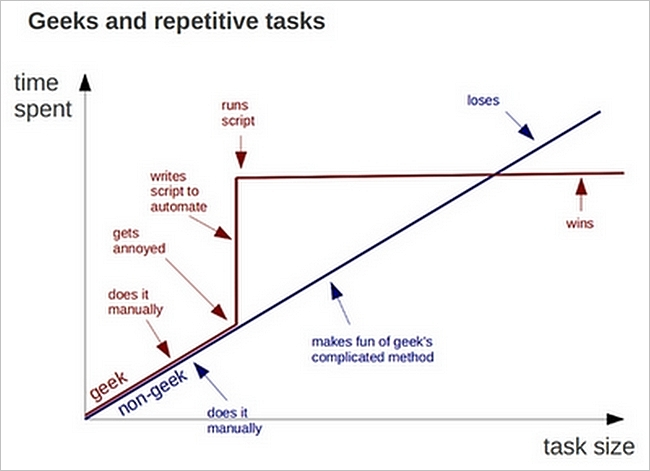
\includegraphics[width=0.75\textwidth]{automated.jpg}
\caption{Why automate?} 
\end{figure} 

\section{Working with data: Read/Write}
The first procedure in almost any program to analyze data will be entering the data into memory -- in our code into the \R\ workspace. Data can be stored in lots of different ways. Accordingly, there are lots of different ways to load data into \R. For instance, you already know you can type in all your data and place them in a vector using the generic ``combine'' function \code{c} as follows.

\begin{knitrout}
\definecolor{shadecolor}{rgb}{0.969, 0.969, 0.969}\color{fgcolor}\begin{kframe}
\begin{alltt}
\hlstd{data.demo}\hlkwb{<-}\hlkwd{c}\hlstd{(}\hlnum{1}\hlstd{,}\hlnum{17}\hlstd{,}\hlnum{4}\hlstd{,}\hlnum{6}\hlstd{)}   \hlcom{#create a data vector}
\hlstd{data.demo}
\end{alltt}
\begin{verbatim}
## [1]  1 17  4  6
\end{verbatim}
\end{kframe}
\end{knitrout}

For research purposes, this is very inefficient. It is often most convenient to enter data into a spreadsheet or database management software and then save as comma-separated \emph{flat files} with a ``.csv'' extension. Then, the data are read into \R\ using the function \code{read.csv}. We note that although \R\ has functions for reading (and writing) data in other file formats, for maximum interoprerability it is almost always best to save flat tables (not relational data based) in ascii formatted comma separated files. For instance, data on an outbreak of influenza in a British boarding school have been provided in the file \texttt{flu.csv}.

\begin{exercise}
  To confirm this, open the file \texttt{flu.csv} in a text editor (such as Notepad) and a speadsheet program (such as Microsoft Excel). Describe what you see.
\end{exercise}

To read a comma separated data file, use the function \code{read.csv}. For example:

\begin{knitrout}
\definecolor{shadecolor}{rgb}{0.969, 0.969, 0.969}\color{fgcolor}\begin{kframe}
\begin{alltt}
\hlstd{flu} \hlkwb{<-} \hlkwd{read.csv}\hlstd{(}\hlstr{'flu.csv'}\hlstd{)}
\end{alltt}
\end{kframe}
\end{knitrout}

To print the resulting dataframe to the console just enter the name of the data object.

\begin{knitrout}
\definecolor{shadecolor}{rgb}{0.969, 0.969, 0.969}\color{fgcolor}\begin{kframe}
\begin{alltt}
\hlstd{flu}
\end{alltt}
\begin{verbatim}
##    day flu
## 1    1   3
## 2    2   8
## 3    3  28
## 4    4  76
## 5    5 222
## 6    6 293
## 7    7 257
## 8    8 237
## 9    9 192
## 10  10 126
## 11  11  70
## 12  12  28
## 13  13  12
## 14  14   5
\end{verbatim}
\end{kframe}
\end{knitrout}

Just as we can read a comma separated data file, \R\ also allows one to save a dataframe to a comma separated data file using the function \code{write.csv}.

\begin{exercise}
  To use \texttt{write.csv} one needs to know what arguments to provide. Review the help files for \code{write.csv} and save the flu data frame to a new file \texttt{flu-2.csv}. View \texttt{flu-2.csv} in a text editor. How is \texttt{flu-2.csv} different than the original file \texttt{flu.csv}?
\end{exercise}

Comma separated files are in general a great way to save flat data tables and other simple data structures. But, in a typical \R\ session one might create a lot of different objects. It would be quite unwieldy to save all of them as separate files, right? Fortunately, \R\ provides for this possibility by allowing one to save an entire \R\ workspace, that is all the objects in memory at some point in a session. These files are assigned the ``R data'' format and end with either suffix \texttt{.RData} or \texttt{.rda}. For this class, we have provided four different datasets all stored together in a single \R\ workspace. After clearing the workspace to remove the old \code{flu} object, these may be loaded into memory with the \code{load} function. (Note that \code{flu} is included in the data sets in \texttt{data.RData})

\begin{knitrout}
\definecolor{shadecolor}{rgb}{0.969, 0.969, 0.969}\color{fgcolor}\begin{kframe}
\begin{alltt}
\hlkwd{rm}\hlstd{(}\hlkwc{list}\hlstd{=}\hlkwd{ls}\hlstd{(}\hlkwc{all}\hlstd{=}\hlnum{TRUE}\hlstd{))}    \hlcom{# clear workspace}
\hlkwd{load}\hlstd{(}\hlstr{'data.RData'}\hlstd{)}       \hlcom{# load data sets}
\end{alltt}
\end{kframe}
\end{knitrout}

\begin{challenge}
  Explain how the line \code{rm(list=ls(all=TRUE))} works.
\end{challenge}

\begin{challenge}
  What would have happened if we have not cleared the workspace before loading the new data? How can you check?
\end{challenge}

\section{Plotting}

Now that the data have been read into memory, they are available for use. To see everything that's in memory at the present time, enter
the command \code{ls()}. As above, we can inspect the influenza dataset by typing its name into the console.

\begin{knitrout}
\definecolor{shadecolor}{rgb}{0.969, 0.969, 0.969}\color{fgcolor}\begin{kframe}
\begin{alltt}
\hlstd{flu}
\end{alltt}
\begin{verbatim}
##    day flu
## 1    1   3
## 2    2   8
## 3    3  28
## 4    4  76
## 5    5 222
## 6    6 293
## 7    7 257
## 8    8 237
## 9    9 192
## 10  10 126
## 11  11  70
## 12  12  28
## 13  13  12
## 14  14   5
\end{verbatim}
\end{kframe}
\end{knitrout}

What do the data represent? These data are from an outbreak of influenza in a British boarding school in 1978 (Anonymous 1978). There is a unique entry in the variable \code{day} for each day of the outbreak. The variable \code{flu} contains the corresponding number of boys confined to bed. We can plot these data using the following command.

\begin{knitrout}
\definecolor{shadecolor}{rgb}{0.969, 0.969, 0.969}\color{fgcolor}\begin{kframe}
\begin{alltt}
\hlkwd{plot}\hlstd{(flu}\hlopt{$}\hlstd{day,flu}\hlopt{$}\hlstd{flu,} \hlkwc{type}\hlstd{=}\hlstr{'b'}\hlstd{,}\hlkwc{xlab}\hlstd{=}\hlstr{'Day'}\hlstd{,}\hlkwc{ylab}\hlstd{=}\hlstr{'Number of individuals infected'}\hlstd{)}
\end{alltt}
\end{kframe}
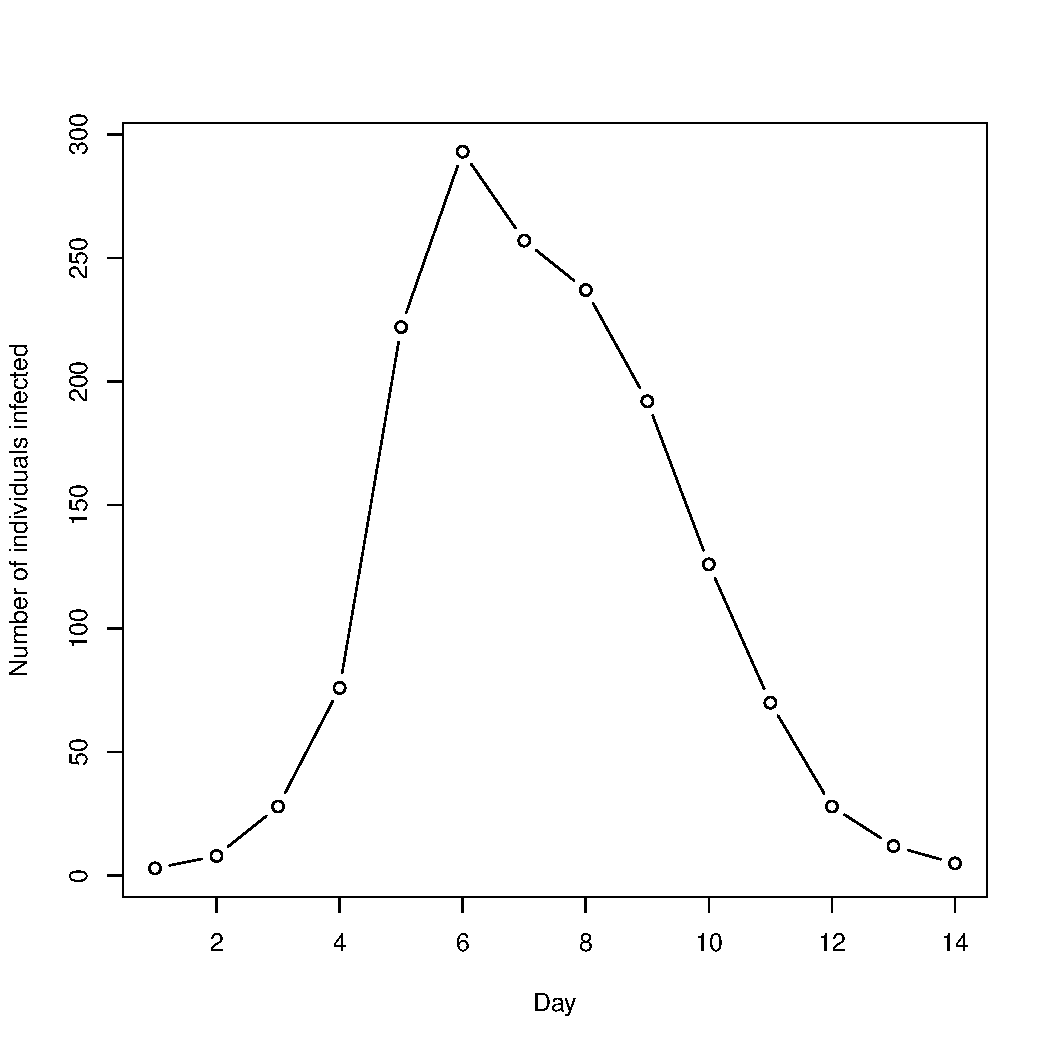
\includegraphics[width=\maxwidth]{figure/unnamed-chunk-6-1} 

\end{knitrout}

We  learn a number of things by studying this code. First, a single variable can be referenced by typing the name of the data frame (e.g., \code{flu}) followed by the name of a variable (e.g., \code{day}) separatated by a dollar sign. This allows us to extract, manipulate, assign variables independently. For instance, the following lines creates a new object (a vector), called \code{prevalence}, by extracting flu cases and dividing through by a presumed population size of 764 (763 boys ``at risk'' plus index case).

\begin{knitrout}
\definecolor{shadecolor}{rgb}{0.969, 0.969, 0.969}\color{fgcolor}\begin{kframe}
\begin{alltt}
\hlstd{prevalence}\hlkwb{<-}\hlstd{flu}\hlopt{$}\hlstd{flu}\hlopt{/}\hlnum{764}
\hlstd{prevalence}
\end{alltt}
\begin{verbatim}
##  [1] 0.003926702 0.010471204 0.036649215 0.099476440 0.290575916
##  [6] 0.383507853 0.336387435 0.310209424 0.251308901 0.164921466
## [11] 0.091623037 0.036649215 0.015706806 0.006544503
\end{verbatim}
\end{kframe}
\end{knitrout}

The next thing to notice about our plot command is that the first two arguments are not names. Rather, \code{plot} just assumed that the first two arguments should be placed on the x-axis and y-axis respectively. If we switch the sequence, we obtain the following plot.

\begin{knitrout}
\definecolor{shadecolor}{rgb}{0.969, 0.969, 0.969}\color{fgcolor}\begin{kframe}
\begin{alltt}
\hlkwd{plot}\hlstd{(flu}\hlopt{$}\hlstd{flu,flu}\hlopt{$}\hlstd{day,} \hlkwc{type}\hlstd{=}\hlstr{'b'}\hlstd{,}\hlkwc{xlab}\hlstd{=}\hlstr{'Day'}\hlstd{,}\hlkwc{ylab}\hlstd{=}\hlstr{'Number of individuals infected'}\hlstd{)}
\end{alltt}
\end{kframe}
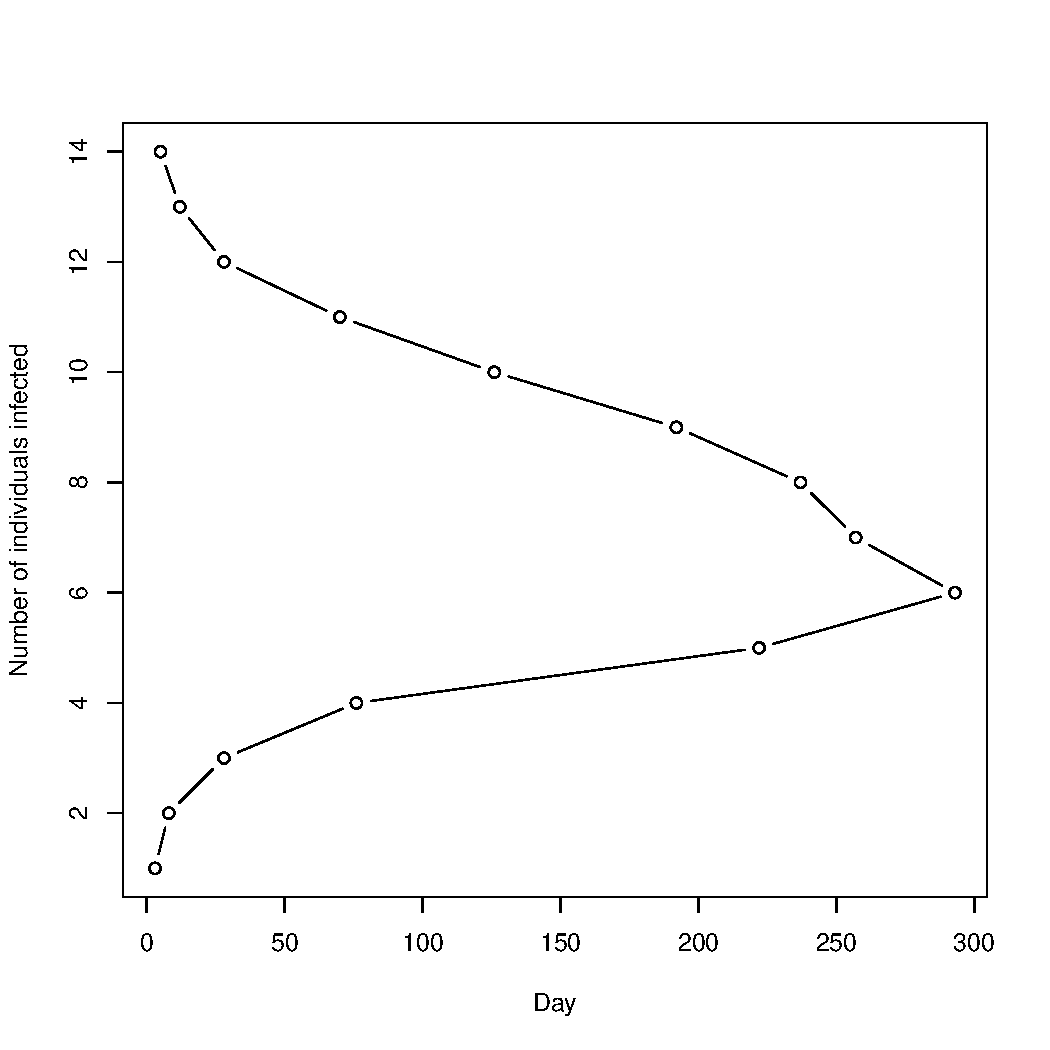
\includegraphics[width=\maxwidth]{figure/unnamed-chunk-8-1} 

\end{knitrout}

Alternatively, the order doesn't matter if we specify which value is which argument, \textit{i.e.}, the following line reproduces the original plot even though the x and y arguments are out of sequence.


\begin{knitrout}
\definecolor{shadecolor}{rgb}{0.969, 0.969, 0.969}\color{fgcolor}\begin{kframe}
\begin{alltt}
\hlkwd{plot}\hlstd{(}\hlkwc{y}\hlstd{=flu}\hlopt{$}\hlstd{flu,}\hlkwc{x}\hlstd{=flu}\hlopt{$}\hlstd{day,} \hlkwc{type}\hlstd{=}\hlstr{'b'}\hlstd{,}\hlkwc{xlab}\hlstd{=}\hlstr{'Day'}\hlstd{,}\hlkwc{ylab}\hlstd{=}\hlstr{'Number of individuals infected'}\hlstd{)}
\end{alltt}
\end{kframe}
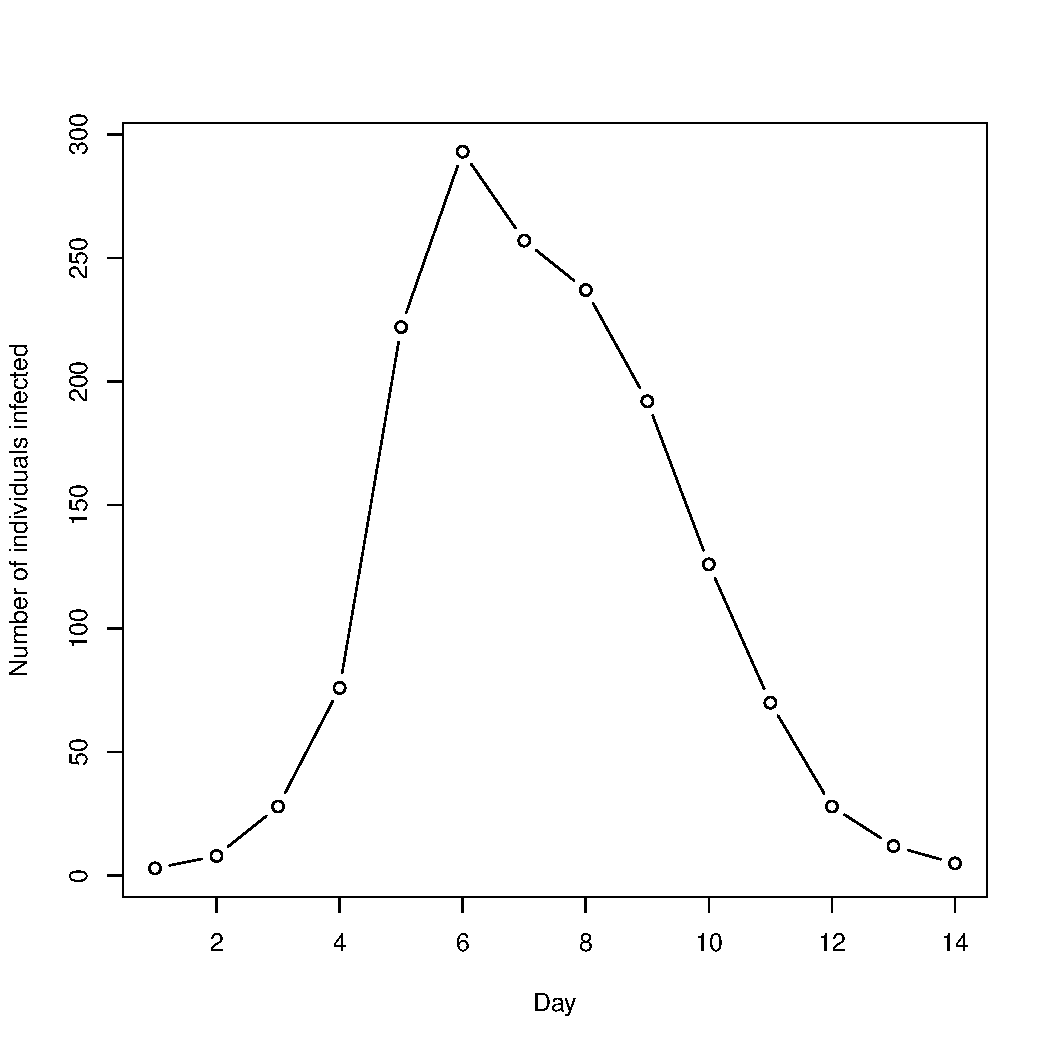
\includegraphics[width=\maxwidth]{figure/unnamed-chunk-9-1} 

\end{knitrout}

In general, it is a good habit to specify each argument, rather than rely on the implicitly expected sequence. For more information on good coding practices see: \url{http://google-styleguide.googlecode.com/svn/trunk/Rguide.xml}

Finally, we see that \code{plot} may take additional arguments (indeed, many more arguments than those used here are possible). Here we specify the type of plot and labels for the x and y axes.

\begin{exercise}
 The plots generated above consist of 'b'oth \emph{points} and \emph{lines}, hence the argument \code{type='b'}. Retrieve the help 
 for the plot function and try some of the other plot types, e.g., line plot and point plot.  
\end{exercise}

The function \code{plot} is intended only for producing scatterplots (in several flavors). Other functions are available for other kinds of plots, including \code{hist} to generate histograms and \code{boxplot} to generate box and whisker plots. Additionally, all aspects of the image may be manipulated (e.g., line thickness (argument \code{lwd}, which takes a numerical value), colors (argument \code{col}), fonts, etc.) with greater or lesser difficulty depending on how deeply related they are to the plots design. Also, lines and points may be added to an existing plot using the functions \code{lines} and \code{points}, respectively.

\begin{exercise}
  Experiment with the functions \code{plot}, \code{lines}, and \code{points} by plotting the measles incidence data from three different districts in the city of Niamey, Niger in different colors on the same figure.
\end{exercise}

\begin{exercise}
  Save the figure from the previous exercise as a pdf using 2 different methods. View them in a pdf viewer, is there a difference in the figures?
\end{exercise}

The function \code{plot} can take a great many additional arguments. Some of these are listed under the help page for \code{plot} (type \code{?plot}); others are not. Those that are listed include \code{main}, \code{sub}, \code{xlab}, and \code{ylab}, which can be assigned character strings to serve as plot titles and subtitles and axis titles. The preceding examples with the \code{flu} data set illustrate usage. Some useful arguments that are not included in the help page are \code{xlim} and \code{ylim}, which allow the programmer to specify the x-axis and y-axis limits, which are referenced by a two-element vector (e.g. \code{ylim=c(-10, 100)}). Similarly, the argument \code{log} allows one to specify that the x-axis, y-axis, or both should be on a logarithmic scale, using the arguments \code{log='x'}, \code{log='y'}, and \code{log='xy'}, respectively. If using symbols in plotting (e.g. for \code{plot} where \code{type='p'} or \code{type='b'}), any of a large number of symbols are available by specifying the argument \code{pch}. For a more complete description and list of available symbols (some of which are two-color) type \code{?pch}. The size of the symbol and/or axis titles may be adjusted using \textit{character expansion} (argument \code{cex}), a factor by which to increase or decrease the size of the symbols. Thus, the argument \code{cex=2} increases the symbol size two fold whereas \code{cex=0.5} decreases it by half.

\section{Descriptive statistcs}

\textit{Descriptive statistics} refers to statistical methods used to summarize data. Quantities like the \textit{mean} (average), \textit{variance} and \textit{standard deviation} (measures of data dispersion), and \textit{minimum} or \textit{maximum} (measures of extremes) are descriptive statistics. We will use the data on measles from three districts in Niamey, Niger to illustrate these methods. Measles is an acute immunizing infection with an approximately 14 day infectious period. For this reason, epidemiological studies of measles often aggregate cases to a biweekly interval. That is, each row of the data frame corresponds to a 14 day period. To calculate the average number of cases in the first district over the entire course of the epidemic, we use the following command:

\begin{knitrout}
\definecolor{shadecolor}{rgb}{0.969, 0.969, 0.969}\color{fgcolor}\begin{kframe}
\begin{alltt}
\hlkwd{mean}\hlstd{(niamey[,}\hlnum{1}\hlstd{])}
\end{alltt}
\begin{verbatim}
## [1] 370.6875
\end{verbatim}
\end{kframe}
\end{knitrout}

Alternatively, we can calculate the average number just during the peak (weeks 15 to 25 or biweeks 8 to 13) by referencing just those entries we are interested in.

\begin{knitrout}
\definecolor{shadecolor}{rgb}{0.969, 0.969, 0.969}\color{fgcolor}\begin{kframe}
\begin{alltt}
\hlkwd{mean}\hlstd{(niamey[}\hlnum{8}\hlopt{:}\hlnum{13}\hlstd{,}\hlnum{1}\hlstd{])}
\end{alltt}
\begin{verbatim}
## [1] 828
\end{verbatim}
\end{kframe}
\end{knitrout}

Suppose we wish to calculate across districts, say we wish to know the average number of measles cases during weeks 13 and 14 (biweek number 7) over the entire city. For this, we issue the following command:

\begin{knitrout}
\definecolor{shadecolor}{rgb}{0.969, 0.969, 0.969}\color{fgcolor}\begin{kframe}
\begin{alltt}
\hlkwd{mean}\hlstd{(}\hlkwd{as.numeric}\hlstd{(niamey[}\hlnum{7}\hlstd{,]))}
\end{alltt}
\begin{verbatim}
## [1] 100.3333
\end{verbatim}
\end{kframe}
\end{knitrout}

Note that since \code{niamey} is a data.frame, \R\ doesn't think of its rows as being vectors of numbers. Accordingly, we have to coerce these numbers to a vector using the function \code{as.numeric}. You may find from time to time that the function for some procedure (here it is calculating the mean) cannot be applied to your object. In these cases, obtaining the desired outcome may require two steps: (1) making an object of the right kind (data frame, list, vector, etc.) containing the target information, then (2) performing the procedure. Fortunately, \R\ has lots of functionality for coercing objects of one kind to another and back again.

Finally, look again at the data for the third district in Niamey. 

\begin{knitrout}
\definecolor{shadecolor}{rgb}{0.969, 0.969, 0.969}\color{fgcolor}\begin{kframe}
\begin{alltt}
\hlstd{niamey[,}\hlnum{3}\hlstd{]}
\end{alltt}
\begin{verbatim}
##  [1]   0   0   0   2  NA   4   3  20  49  81 116 164 159  33  16   5
\end{verbatim}
\end{kframe}
\end{knitrout}

For some reason, data are missing for weeks 9 and 10 (biweek 5). The originators of this data set were correct to score this as \code{NA} rather than zero -- it's not zero cases after all. But, \code{NA} is also not a number. How do we calculate a summary statistic of numers that contain missing values? This is especially important for population data and other surveillance data that may not be collected consistently over the entire study period. For staters, we can try and calculate the mean number of cases in the third Niamey district.

\begin{knitrout}
\definecolor{shadecolor}{rgb}{0.969, 0.969, 0.969}\color{fgcolor}\begin{kframe}
\begin{alltt}
\hlkwd{mean}\hlstd{(niamey[,}\hlnum{3}\hlstd{])}
\end{alltt}
\begin{verbatim}
## [1] NA
\end{verbatim}
\end{kframe}
\end{knitrout}

The result is, again, \code{NA}. This is an \R\ convention: the mean of a series of numbers containing \code{NA}'s is itself \code{NA}. So, that's fine as far as it goes, but suppose instead we want to know the average number of measles cases in the third district \textit{during intervals when the data was collected}. How do we calculate that? The answer, use the additional argument \code{na.rm=TRUE} to indicate that any \code{NA}'s should be \textit{removed} prior to performing the calculation.

\begin{knitrout}
\definecolor{shadecolor}{rgb}{0.969, 0.969, 0.969}\color{fgcolor}\begin{kframe}
\begin{alltt}
\hlkwd{mean}\hlstd{(niamey[,}\hlnum{3}\hlstd{],} \hlkwc{na.rm}\hlstd{=}\hlnum{TRUE}\hlstd{)}
\end{alltt}
\begin{verbatim}
## [1] 43.46667
\end{verbatim}
\end{kframe}
\end{knitrout}

\begin{exercise}
Scoring missing values as \code{NA} is different than treating them as zero. Numerically show this to be the case using the data on measles in the third Niameyt distrct.
\end{exercise}

\begin{exercise}
Practice using other descriptive statistics. First, numerically find in which biweek/district combination the greatest number of cases were reported. Second, determine in which biweek there was the greatest dispersion among cases. Visually verify your results by plotting. 
\end{exercise}

\begin{exercise}
Now, try using the \code{apply} function to repeat the previous exercise. 
\end{exercise}

Finally, as the last task in this section we introduce a new \R\ function: \code{summary}. This function is different than probably almost all the other functions introduced so far in that what it does depends on the nature of the object it is applied to. When that object is a data frame, what it does is return a descriptive summary of the variables contained in the data frame. For instance:

\begin{knitrout}
\definecolor{shadecolor}{rgb}{0.969, 0.969, 0.969}\color{fgcolor}\begin{kframe}
\begin{alltt}
\hlkwd{summary}\hlstd{(niamey)}
\end{alltt}
\begin{verbatim}
##        V1                V2               V3        
##  Min.   :  11.00   Min.   :  1.00   Min.   :  0.00  
##  1st Qu.:  78.25   1st Qu.: 16.75   1st Qu.:  2.50  
##  Median : 172.50   Median : 98.00   Median : 16.00  
##  Mean   : 370.69   Mean   :271.62   Mean   : 43.47  
##  3rd Qu.: 755.25   3rd Qu.:548.25   3rd Qu.: 65.00  
##  Max.   :1041.00   Max.   :874.00   Max.   :164.00  
##                                     NA's   :1
\end{verbatim}
\end{kframe}
\end{knitrout}

Later, we will see another use for \code{summary}.

\section{Inferential statistics}

\subsection{t-test}

Whereas descriptive statistics is concerned with calculating numerical summaries, inferential statistics is concerned with the \textit{evidence} for or against certain ideas. Inferential statistics is the branch of statistics that deals with \textit{hypthesis tests}. If you have taken courses in probability and statistics, you may recall concepts such as \textit{p-values}, \textit{F statistics}, \textit{z-scores}, and \textit{confidence intervals}. These are part of inferential statistics. Of course, \R\ is able to calculate these things and, indeed, a great many other quantities that are useful for scientific inference as well.

To start, we'll consider the problem of testing for a \textit{difference of means}. The problem is this: suppose we have two different sets of observations and we would like to know if these sets are different from each other, or if the numerical differences we see are simply based on sampling error. For our purposes, we may wonder if the number of average cases in the three districts of Niamey are different from each other. (Note that we are only asking \textit{if} they are different, not \textit{why} they are different. If we find that they are in fact different, there still may be many reasons for this: one district or another may have higher prevalence, or the districts may just be different in overall size, etc.). Conventionally, we will say that ``no difference'' is the \textit{null hypothesis} and ``there is a difference'' is the \textit{alternate hypothesis}. We seek to ``reject'' the null hypothesis and the traditional statistical test is the t-test. In \R, a t-test may be performed using the function \code{t.test}. Thus, to test for a difference of means between Niamey district 1 and Niamey district 2, we issue the following command:

\begin{knitrout}
\definecolor{shadecolor}{rgb}{0.969, 0.969, 0.969}\color{fgcolor}\begin{kframe}
\begin{alltt}
\hlkwd{t.test}\hlstd{(niamey[,}\hlnum{1}\hlstd{], niamey[,}\hlnum{2}\hlstd{])}
\end{alltt}
\begin{verbatim}
## 
## 	Welch Two Sample t-test
## 
## data:  niamey[, 1] and niamey[, 2]
## t = 0.7976, df = 29.273, p-value = 0.4315
## alternative hypothesis: true difference in means is not equal to 0
## 95 percent confidence interval:
##  -154.8592  352.9842
## sample estimates:
## mean of x mean of y 
##  370.6875  271.6250
\end{verbatim}
\end{kframe}
\end{knitrout}

As you see, the result consists of a list of different quantities. We will focus on just two. First, the \textit{95\% confidence interval on the difference of means} consists of two numbers -- a lower confidence limit and an upper confidence limit. This interval has the interpretation that were this operation to be repeated multiple times with different data sets, in 95\% of cases the reported interval would contain the true value of the quantity of interest, in this case the difference between the (true, not estimated) mean number of cases in Niamey district 1 and Niamey district 2. This is a technical definition, which you may be familiar with if you have studied probability and statistics. If you have not studied probability and statistics you can roughly interpret the result this way: any of the values in the interval are broadly consistent with the observed data. Inspecting this confidence interval, we see that it is possible that the true average number of cases in district 1 exceeded the average number in district 2 by as much as 353 cases, that the average number of cases in district 2 exceeded the average number of cases in district 1 by as much as 155 cases (so the difference of means is -155), and everything in between. Since zero is on the interval from -155 to 352, we cannot reject the null hypothesis that there was no difference in the average number of cases in these two districts.

This conclusion is underscored by the p-value, in this case $p=0.4315$. The p-value can be interpreted this way. Suppose the null hypothesis were true, given the sampling variation inherent in these data, what is the probability that a difference of means this great or greater would be observed? For our example, the probability is $\approx 0.43$, almost a 50\% chance. One says that a result is \textit{statistically significant} only when the probability of observing such a case by chance is very small, which we name with the Greek letter $\alpha$ and call the \textit{significance level}. Conventionally, $\alpha$ is chosen to be 5\% or 0.05, so we would say ``this test fails to reject the null hypothesis of no difference at the $\alpha=0.05$ level of significance.

\begin{exercise}
Test for differences in the mean number of cases between districts 1 and 3 and between districts 2 and 3. How do you interpret these results?
\end{exercise}

\subsection{Correlation and linear regression}

Two further techniques for statistical inference are \textit{linear regression} and \textit{correlation}. Correlation considers the level of association between two variables. As an example, the following three plots show three pairs of observations $x_1$ and $x_2$ that differ in their degree of correlation. (Traditionally, the correlation coefficient is named with the Greek letter $\rho$.)

\begin{knitrout}
\definecolor{shadecolor}{rgb}{0.969, 0.969, 0.969}\color{fgcolor}\begin{kframe}


{\ttfamily\noindent\itshape\color{messagecolor}{\#\# Loading required package: mvtnorm}}\end{kframe}
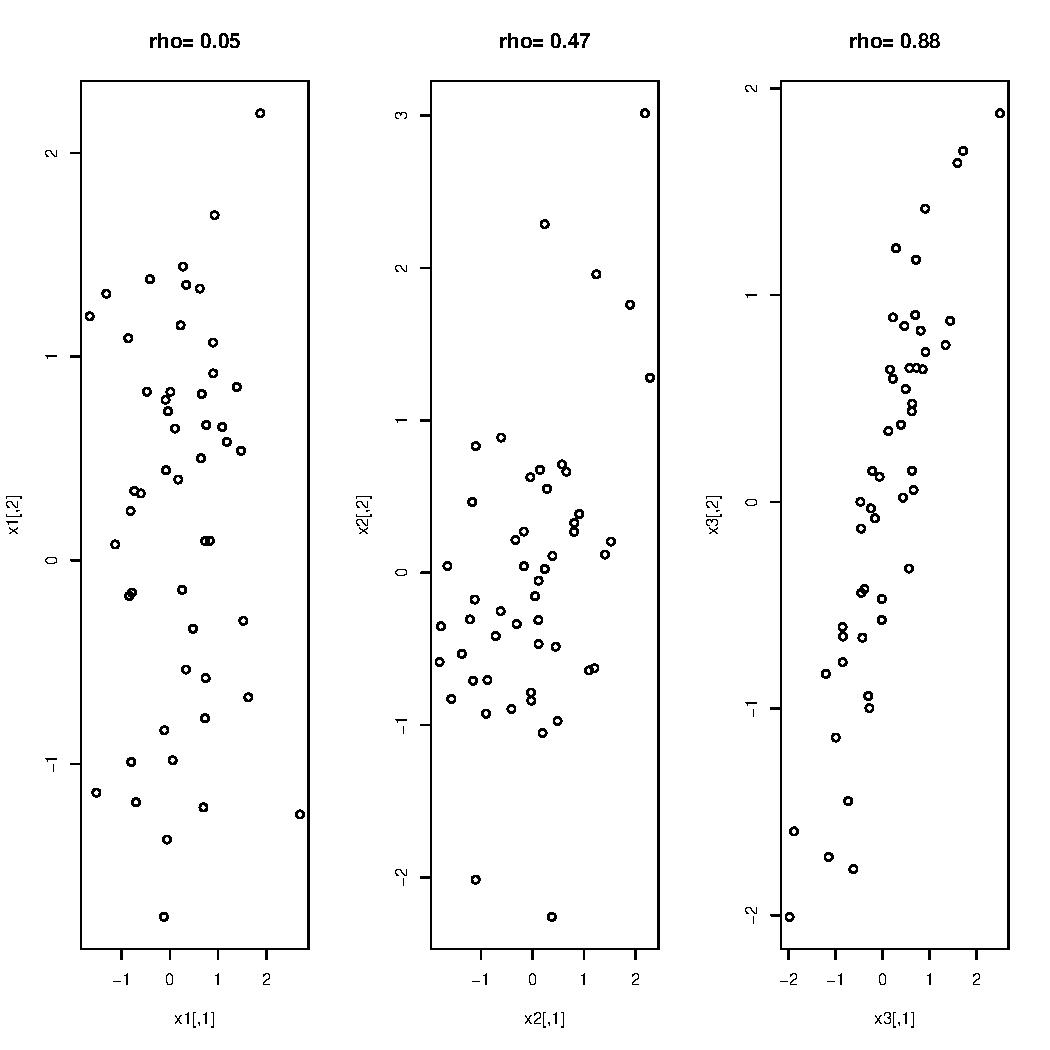
\includegraphics[width=\maxwidth]{figure/unnamed-chunk-18-1} 

\end{knitrout}

From one point of view, correlation is just a descriptive statistic and any two vectors of numbers will have some correlation coefficient. However, in the tradiation hypothesis testing way, we can also express the null hypothesis of no correlation ($H_0: \rho=0$), which we then seek to reject. In \R\, this is done using the function \code{cor.test}, which returns a 95\% confidence interval and a p-value, just as \code{t.test} did to test for a difference of means.

\begin{exercise}
Test for a correlation in the number of cases reported in Niamey districts 1 and 2. Explain your result.
\end{exercise}

\begin{challenge}
The default measure of association returned by \code{cor.test} is called \textit{Pearson's correlation coefficient}. However, there are actually several different conceptions of correlation which differ in technical ways. Another of these is called \textit{Spearman's rank-order coefficient} and may be calculated by using the argument \code{method='spearman'}. Can you surmise how Spearman's correlation differs from Pearson's. Devise a means to calculate Spearman's correlation coefficient without using the argument \code{method='spearman'}.)
\end{challenge}

\subsection{Linear regression}
Linear regression is closely related to Spearman's correlation and also considers the relationship between two variables. Specifically, linear regression assumes that the relationship between two quantities can be represented by a line (which is expressed with the equation $y=mx_i+b$) and that the failure of the data to fall exactly on a line is because of some variation or measurement error in the variable $y$ such that the $i^{th}$ observation $y_i$ can be expressed as $y_i=mx+b+\epsilon_i$, where $\epsilon_i$ is the measurement error. Now, the problem is to find the values of $m$ and $b$ (the slope and intercept) such that the total error is minimized in some sense and possibly also to test hypothesis (for instance that $m=0$ or $b=0$). In ordinary (least squares) regression, we seek to minimize the \textit{sum of squared errors}: $\Sigma_i (y_i-(mx_i+b))^2$. Since this is a \textit{linear model}, the best fitting values of $m$ and $b$, as well as a lot of other information, may be obtained using the function \code{lm}.

To illustrate, we draw on a piece of epidemiological theory. By way of background, theoretical epidemiologists are often concerned with a key quantity called the \textit{basic reproduction ratio}, designated $R_0$. $R_0$ is defined as the average number of secondary cases that will arise by contagious infection from an index patient in a wholly susceptible popuation. $R_0=1$ is known as a critical point because infectious diseases with $R_0>1$ almost always result in large epidemics whereas infectious diseases with $R_0<1$ rapidly die out. (Do you see why this is, given the definition?) It can be shown (using arguments not reproduced here) that for a rapidly spreading epidemic

\begin{equation*}
  \log{Y_t}\;\approx\;\log{Y_0}+(R_0-1)\,(\gamma)\,t, 
\end{equation*}

where $Y_t$ is the number of individuals currently infected at time $t$ and $\gamma^{-1}$ is the \textit{infectious period}. This implies that a semi-log plot of $Y_t$ vs $t$ should be approximately linear with a slope proportional to $R_0-1$ and the recovery rate. If we plot the influenza data, we see that this is indeed the case.

\begin{knitrout}
\definecolor{shadecolor}{rgb}{0.969, 0.969, 0.969}\color{fgcolor}\begin{kframe}
\begin{alltt}
\hlkwd{plot}\hlstd{(flu,} \hlkwc{type}\hlstd{=}\hlstr{'b'}\hlstd{,} \hlkwc{log}\hlstd{=}\hlstr{'y'}\hlstd{,} \hlkwc{xlab}\hlstd{=}\hlstr{'Day'}\hlstd{,} \hlkwc{ylab}\hlstd{=}\hlstr{'Number of individuals infected'}\hlstd{)}
\end{alltt}
\end{kframe}
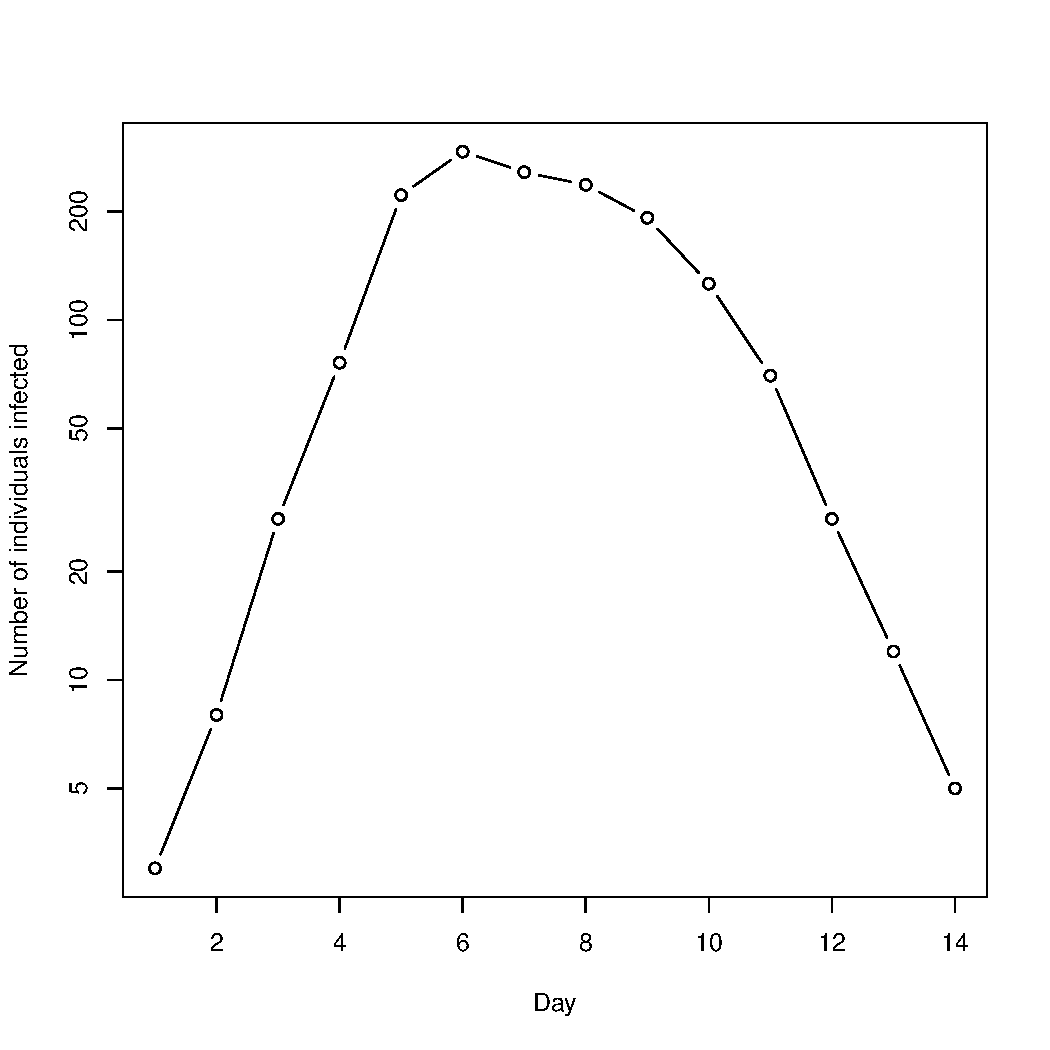
\includegraphics[width=\maxwidth]{figure/unnamed-chunk-19-1} 

\end{knitrout}

Ultimately, then, linear regression will allow us to estimate $R_0$. However, to do this we need to note a few things. First, it is the logarithm of the number of cases on day $t$ that takes the place of $y$ in our expression $y=mx+b$. In \R\ the logarithm is calculated using the function \code{log}. Next, $log(Y_0)$ takes the place of $b$. If we assume that the epidemic was started by a single infectious individual, then $b=log(1)=0$, so we're interested not in any best fitting line, but only that best fit line that also goes through $(x=0, y=0)$. In regression analysis, this is called fitting a model \textit{without an intercept}. Third, if we interpret $t$ as the quantity that take the place of $x$ in $y=mx+b$, then we see that it is the entire expression $(R_0-1)\,(\gamma)$ that forms the slope $m$. Finally, the formula only applies to the \textit{epidemic takeoff}, so we only want to fit a subset of our data. Inspecting the plot suggests that we might fit our line to data for all days up to and including day 5 of the outbreak. Now, we fit the line using \code{lm} as follows:

\begin{knitrout}
\definecolor{shadecolor}{rgb}{0.969, 0.969, 0.969}\color{fgcolor}\begin{kframe}
\begin{alltt}
\hlstd{model} \hlkwb{<-} \hlkwd{lm}\hlstd{(}\hlkwc{formula}\hlstd{=}\hlkwd{log}\hlstd{(flu)}\hlopt{~}\hlstd{day}\hlopt{-}\hlnum{1}\hlstd{,}\hlkwc{data}\hlstd{=}\hlkwd{subset}\hlstd{(flu,day}\hlopt{<=}\hlnum{5}\hlstd{))}
\end{alltt}
\end{kframe}
\end{knitrout}

Before looking at the output, there are a number of things to notice about this command. First, the results are stored in an object that I have called \code{model}. Second, the first argument (called \code{formula}) is nothing like any argument we've seen before. It looks sort of like a mathematical expression. the first term says that the quantity which we want to take the place of $y$ in our formula $y=mx+b$ is the logarithm of something called ``flu''. (But where does ``flu'' come from? More on that in a moment.) Next we see the character tilde ($\sim$). This may be read as ``distributed as'' or you may more simply think of this as taking the place of the equals sign in our formula $y=mx+b$. Finally, to the right of tilde we see information about what is on the right hand side of the equation. First, there is ``day'', which takes the place of $x$. (But where does ``day'' come from? Answer: the same place as ``flu''.) Because ``day'' is a variable, \R\ assumes you wish to find a slope parameter to multiply by ``day''. Finally, we also see that there is a $-1$, which is a coded way of telling \R\ that we wish to fit only equations that go through the origin. If we left this off, \R\ would seek to find a combination of $m$ and $b$ that minimized the sum of squared errors. As it is, \R\ will fix the intercept at zero and return only a slope coefficient. Now, where does \R\ look to find the variables ``flu'' and ``day''? This is provided by the argument \code{data}. The possible values for data are data frames that contain variables called ``flu'' and ``day''. If we supplied the name of a data frame that did not contain these variables \R\ would return an error. In our case, however, we're not interested in using all the data in \code{flu}, but only those records for which ``day'' is less than or equal to 5, which we obtain using the \code{subset} function as indicated.

Now we wish to see what our fit model consists of. For starters, we can simply type the name of the object at the command line.

\begin{knitrout}
\definecolor{shadecolor}{rgb}{0.969, 0.969, 0.969}\color{fgcolor}\begin{kframe}
\begin{alltt}
\hlstd{model}
\end{alltt}
\begin{verbatim}
## 
## Call:
## lm(formula = log(flu) ~ day - 1, data = subset(flu, day <= 5))
## 
## Coefficients:
##   day  
## 1.083
\end{verbatim}
\end{kframe}
\end{knitrout}

This, we see, prints to the screen the formula that was used to fit the model as well as the fit coefficients, in our case $m=1.086$. But, there is more information that we can obtain. Here we come to the other common use of \code{summary}. If we ask for a summary of the model, we see that we get a lot more information: the formula; a list of residuals (the $\epsilon_i$ from above); more information about the coefficient $m$, including the estimate, an estimate of its error (i.e. a value that when we add and substract to the estimate provides an interval -- though not a 95\% confidence interval), something called the ``t-value'' (which we won't worry about more), and finally a p-value for the hypothesis test that the coefficient is equal to zero. Also, we get some additional summary statistics such as the $R^2$ value (fraction of variance explained by the model) and other statistical details.

\begin{knitrout}
\definecolor{shadecolor}{rgb}{0.969, 0.969, 0.969}\color{fgcolor}\begin{kframe}
\begin{alltt}
\hlkwd{summary}\hlstd{(model)}
\end{alltt}
\begin{verbatim}
## 
## Call:
## lm(formula = log(flu) ~ day - 1, data = subset(flu, day <= 5))
## 
## Residuals:
##         1         2         3         4         5 
##  0.015150 -0.087483  0.081817 -0.003116 -0.014634 
## 
## Coefficients:
##     Estimate Std. Error t value Pr(>|t|)    
## day 1.083462   0.008202   132.1 1.97e-08 ***
## ---
## Signif. codes:  0 '***' 0.001 '**' 0.01 '*' 0.05 '.' 0.1 ' ' 1
## 
## Residual standard error: 0.06083 on 4 degrees of freedom
## Multiple R-squared:  0.9998,	Adjusted R-squared:  0.9997 
## F-statistic: 1.745e+04 on 1 and 4 DF,  p-value: 1.97e-08
\end{verbatim}
\end{kframe}
\end{knitrout}

Finally, then, we are in a position to calculate $R_0$. Recalling from before, we understand that there is an equivalence between $m$ in the equation $y=mx+b$ and the parameter combination $(R_0-1) \gamma$ so we write $m=(R_0-1) \gamma$. Given that the infectious period of influenza is about 2.5 days, we conclude that $\gamma \approx 2.5^{-1} = 0.4$. Rearraging, we have $\hat{R_0} = m/ \gamma +1 = 1.0895 / 0.4 + 1 \approx 3.7$ (writing $R_0$ with a ``hat'' to signify that this is an estimate).

\begin{exercise}
Estimate $R_0$ for measles in the three districts of Niamey.
\end{exercise}

\section*{Bibliography}

Anonymous. 1978. Influenza in a boarding school. \textit{British Medical Journal} 1:587.

% 
% \section{Random number generation}
% 
% We conclude this session with an introduction to (pseudo-) random number generation in \R.  Both statistical analysis and numerical simulation can require random number generation and \R\ is enabled to generate random numbers from  any of a large number of distributions, including beta, binomial, Cauchy, chi-squared, exponential, Fisher, gamma, geometric, hypergeometric, logistic, lognormal, negative binomial, normal (Gaussian), Poisson, Student t, uniform, and Weibull. Each of these distributions has an abbreviated ``code name''. For instance, for the normal distribution it is \code{norm} and for the uniform it is \code{unif}. Generating random numbers with these distributions is achived by prefixing the code name with the letter ``r'' so that generation of uniform random numbers is done with the function \code{runif}, generation of normally distributed random numbers is done with the function \code{rnorm}, and so forth. When used, the first argument will be the number of random numbers to be generated.  Other arguments are the parameters of the distribution. So, for example, the following code generates 3 random numbers from a normal distribution with mean 5 and standard deviation 3.
% 
% <<>>=
% random.numbers<-rnorm(3,mean=5,sd=3)
% random.numbers
% @ 
% 
% In a later session we will generate random numbers from the exponential distribution with the function \code{rexp}. This distribution has only
% one parameter, the rate, which is also the reciprocal of the mean.
% 
% \begin{exercise}
% Generate one hundred random numbers and plot a histogram.
% \end{exercise}

\end{document}
